\chapter{Análisis}

Siguiendo las necesidades del cliente sintetizadas en los objetivos[\ref{sec:objetives}] iniciaremos el análisis de los requisitos de la aplicación. Dividiremos la fase de análisis en dos: análisis de los requisitos funcionales y no funcionales \cite{ing_software}.

\section{Análisis de los requisitos funcionales}

Los requisitos funcionales son las características requeridas del sistema que expresan una funcionalidad de este:


\begin{itemize}
	\item \textbf{RF-1.} Consulta de datos de una hoja de cálculo de Google Drive
	\item \textbf{RF-2.} Mostrar conceptos de la asignatura
	\item \textbf{RF-3.} Se deberá generar preguntas aleatorias de cada tema. Las preguntas deberán estar diferenciadas en dos tipos:
		\begin{itemize}
			\item \textbf{RF-3.1.} Generación de pregunta tipo test con varias opciones y sólo una seleccionable.
			\item \textbf{RF-3.2.} Generación de pregunta verdadero/falso.
		\end{itemize}
	\item \textbf{RF-4.} Se deberá generar un examen de 20 preguntas aleatorias del tipo de preguntas seleccionado.
	\item \textbf{RF-5.} Se generarán estadísticas básicas de las actividades realizadas por cada alumno en la aplicación. 
		\begin{itemize}
			\item \textbf{RF-5.1.} Número de preguntas correctas e incorrectas.
			\item \textbf{RF-5.2.} Número de exámenes aprobados y suspendidos.
			\item \textbf{RF-5.3.} Nota media de los exámenes aprobados y suspendidos así como la nota media total.
		\end{itemize}
	\item \textbf{RF-6.} Los profesores podrán consultar las estadísticas de los alumnos.
	\item \textbf{RF-7.} Los profesores podrán actualizar los datos de la aplicación, estos se leerán de la hoja de cálculo de Google Drive.
	\item \textbf{RF-8.} Gestión de los usuarios de la aplicación.
\end{itemize}


\section{Análisis de los requisitos no funcionales}

Los requisitos no funcionales hacen referencia a las cualidades del producto requeridas por el cliente. Estas características no se limitan a la aplicación, pueden ser referentes al sistema, al proceso de desarrollo o incluso al entorno.

\begin{itemize}
  \item \textbf{RNF-1.} Rendimiento. Especial cuidado con la velocidad de carga entre secciones.
  \item \textbf{RNF-2.} Conceptos y preguntas se agruparán por temas.
  \item \textbf{RNF-3.} La aplicación se visualizará desde diversos dispositivos, atender a las diferentes resoluciones de pantalla.
  \item \textbf{RNF-4.} Eficiencia en el uso y descarga de datos. Esto es, por ejemplo, el usuario que consulta la aplicación no deberá descargar todo el contenido de la hoja, sólo deberá descargar los datos de la sección consultada.
\end{itemize}


\section{Casos de uso}
	Los casos de uso son una técnica para especificar el comportamiento de un sistema. Hacen referencia a los procedimientos llevados a cabo entre el sistema y una entidad para dar una funcionalidad. Las entidades que participan en estas interacciones con el sistema se denominan actores.

\subsection{Actores}

	
\begin{itemize}
  \item \textbf{Ac-1. Usuario anónimo.}
  \begin{itemize}
   \item \textbf{Descripción:} Persona que visita la aplicación.
   \item \textbf{Características:} Es el usuario que llega por primera vez a la aplicación.
   \item \textbf{Relaciones:} Ninguna.
   \item \textbf{Atributos:} Ninguno.
   \item \textbf{Comentarios:} Este usuario no puede hacer uso de la aplicación más que ver que actividades se desarrollan o alguna información sobre el proyecto.
  \end{itemize}
\end{itemize}

\begin{itemize}
  \item \textbf{Ac-2. Usuario alumno.}
  \begin{itemize}
   \item \textbf{Descripción:} Persona que ha iniciado sesión en la aplicación.
   \item \textbf{Características:} Es el usuario que puede realizar las actividades docentes de la asignatura.
   \item \textbf{Relaciones:} Ninguna.
   \item \textbf{Atributos:} usuario, contraseña, nombre, apellidos y email.
   \item \textbf{Comentarios:} No tiene permisos de administración.
  \end{itemize}
\end{itemize}

\begin{itemize}
  \item \textbf{Ac-3. Usuario profesor.}
  \begin{itemize}
   \item \textbf{Descripción:} Persona que visita la aplicación.
   \item \textbf{Características:} Usuario con permisos de administración de la información docente.
   \item \textbf{Relaciones:} Ninguna.
   \item \textbf{Atributos:} usuario, contraseña, nombre, apellidos y email.
   \item \textbf{Comentarios:} Podrá consultar las estadísticas generadas de los usuarios alumnos.
  \end{itemize}
\end{itemize}

\begin{itemize}
  \item \textbf{Ac-4. Usuario administrador.}
  \begin{itemize}
   \item \textbf{Descripción:} Es el administrador del sistema.
   \item \textbf{Características:} Usuario que puede gestionar los demás usuarios, así como dar permisos al usuario profesor.
   \item \textbf{Relaciones:} Ninguna.
   \item \textbf{Atributos:} usuario, contraseña y email.
   \item \textbf{Comentarios:} Aunque no se restrinja, este usuario no está destinado al uso de la aplicación más allá de las labores de gestión del sistema.
  \end{itemize}
\end{itemize}


\subsection{Casos de uso}

\begin{itemize}
  \item \textbf{CU-1.} Inicio de sesión en el sistema.
  \begin{itemize}
    \item \textbf{Actores:} Usuario anónimo.
    \item \textbf{Tipo:} Primario, esencial.
    \item \textbf{Referencias:}
    \item \textbf{Precondición:} No tener iniciada una sesión previamente.
    \item \textbf{Postcondición:} El usuario anónimo pasará a ser ususario alumno ó ususario profesor.
    \item \textbf{Autor:} \autor.
    \item \textbf{Versión:} 1.0.
    \item \textbf{Propósito:} Pasar a ser un usuario con la sesión iniciada en el sistema.
    \item \textbf{Resumen:} El usuario introducirá su nombre de usuario y su contraseña para iniciar sesión.

    \end{itemize}
    \begin{table}[!ht]
      \begin{center}
	\begin{tabular}{|l|l|l|l|}
	  \hline
	  \multicolumn{4}{|c|}{{\bf Curso normal}}
	  \\ \hline
	  \multicolumn{2}{|c|}{{\bf Actor}} & \multicolumn{2}{c|}{{\bf Sistema}}
	  \\ \hline
	  {\it 1} & 
	  \begin{tabular}[c]{@{}l@{}}
	    El usuario hace click en el\\
	    botón ``Iniciar sesión''. \\
	  \end{tabular} &
	  &
	  \\ \hline
	  &
	  &
	  {\it 2} &
	  \begin{tabular}[c]{@{}l@{}}
	    El sistema muestra el formulario\\
	    para inicio de sesión. \\
	  \end{tabular}
	  \\ \hline
	  {\it 3} & 
	  \begin{tabular}[c]{@{}l@{}}
	    El usuario rellena los campos del \\
	    formulario y pulsa el botón ``Iniciar sesión''. \\
	  \end{tabular} &
	  &
	  \\ \hline
	  &
	  &
	  {\it 4a} &
	  \begin{tabular}[c]{@{}l@{}}
	    El sistema valida el usuario y\\
	    la contraseña y si ambos están\\
	    bien y coinciden inicia la \\
	    sesión de ususario. \\
	  \end{tabular}
	  \\ \hline
	\end{tabular}
	\caption{CU-1. Inicio de sesión.}
	\label{table:cu_1}
      \end{center}
    \end{table}
    
    \begin{table}[!ht]
      \begin{center}
	\begin{tabular}{|l|l|}
	  \hline
	  \multicolumn{2}{|c|}{{\bf Curso alterno}}
	  \\ \hline
	  {\it 4b} &
	  \begin{tabular}[c]{@{}l@{}}
	    Si algo ha ido mal en la validación  del usuario y contraseña, \\
	    el sistema vuelve al paso 2 de CU-1 (tabla \ref{table:cu_1}).
	  \end{tabular}\\
	  \hline
	\end{tabular}
	\caption{Curso alterno de CU-1. Inicio de sesión.}
	\label{table:cu_1_ca}
      \end{center}
    \end{table}

    \newpage






  \item \textbf{CU-2.} Registro en el sistema.
  \begin{itemize}
    \item \textbf{Actores:} Usuario alumno.
    \item \textbf{Tipo:} Primario, esencial.
    \item \textbf{Referencias:}
    \item \textbf{Precondición:} No tener iniciada una sesión previamente.
    \item \textbf{Postcondición:} El usuario tendrá una cuenta con la que iniciar sesión.
    \item \textbf{Autor:} \autor.
    \item \textbf{Versión:} 1.0.
    \item \textbf{Propósito:} Tener una cuenta de usuario alumno.
    \item \textbf{Resumen:} El usuario rellenará un formulario de registro del sistema y si todo va bien, tendrá una cuenta con la que iniciar sesión.

    \end{itemize}
    \begin{table}[!ht]
      \begin{center}
	\begin{tabular}{|l|l|l|l|}
	  \hline
	  \multicolumn{4}{|c|}{{\bf Curso normal}}
	  \\ \hline
	  \multicolumn{2}{|c|}{{\bf Actor}} & \multicolumn{2}{c|}{{\bf Sistema}}
	  \\ \hline
	  {\it 1} & 
	  \begin{tabular}[c]{@{}l@{}}
	    El usuario hace click en el botón\\
	    ``Registrarse''. \\
	  \end{tabular} &
	  &
	  \\ \hline
	  &
	  &
	  {\it 2} &
	  \begin{tabular}[c]{@{}l@{}}
	    El sistema muestra el formulario\\
	    para registrar un usuario. \\
	    En este formulario se pedirán: \\
	    nombre de usuario, contraseña, e-mail, \\
	    nombre y apellidos.
	  \end{tabular}
	  \\ \hline
	  {\it 3} & 
	  \begin{tabular}[c]{@{}l@{}}
	    El ususario rellena el formulario \\
	    y lo envía con el botón ``Registrar''. \\
	  \end{tabular} &
	  &
	  \\ \hline
	  &
	  &
	  {\it 4a} &
	  \begin{tabular}[c]{@{}l@{}}
	    El sistema valida los datos \\
	    y sin son correctos el sistema \\
	    registra el usuario.\\
	  \end{tabular}
	  \\ \hline
	\end{tabular}
	\caption{CU-1. Inicio de sesión.}
	\label{table:cu_2}
      \end{center}
    \end{table}
    
    \begin{table}[!ht]
      \begin{center}
	\begin{tabular}{|l|l|}
	  \hline
	  \multicolumn{2}{|c|}{{\bf Curso alterno}}
	  \\ \hline
	  {\it 4b} &
	  \begin{tabular}[c]{@{}l@{}}
	    Si algo ha ido mal en la validación  del formulario, \\
	    el sistema vuelve al paso 2 de CU-2 (tabla \ref{table:cu_2}).
	  \end{tabular}\\
	  \hline
	\end{tabular}
	\caption{Curso alterno de CU-2. Registro en el sistema.}
	\label{table:cu_2_ca}
      \end{center}
    \end{table}


\newpage






  \item \textbf{CU-3.} Cerrar sesión.
  \begin{itemize}
    \item \textbf{Actores:} Usuario alumno, usuario profesor, usuario administrador.
    \item \textbf{Tipo:} Primario.
    \item \textbf{Referencias:}
    \item \textbf{Precondición:} Tener una sesión iniciada.
    \item \textbf{Postcondición:} El usuario no tendrá la sesión iniciada.
    \item \textbf{Autor:} \autor.
    \item \textbf{Versión:} 1.0.
    \item \textbf{Propósito:} Cerrar la sesión de un usuario en el sistema.
    \item \textbf{Resumen:} El usuario pulsará el botón de cerrar sesión y el sistema cerrará la misma, volviendo a la pantalla de inicio de sesión paso 2 de CU-1 (tabla \ref{table:cu_1}).

    \end{itemize}
    \begin{table}[!ht]
      \begin{center}
	\begin{tabular}{|l|l|l|l|}
	  \hline
	  \multicolumn{4}{|c|}{{\bf Curso normal}}
	  \\ \hline
	  \multicolumn{2}{|c|}{{\bf Actor}} & \multicolumn{2}{c|}{{\bf Sistema}}
	  \\ \hline
	  {\it 1} & 
	  \begin{tabular}[c]{@{}l@{}}
	    El usuario hace click en el botón\\
	    ``Cerrar sesión''. \\
	  \end{tabular} &
	  &
	  \\ \hline
	  &
	  &
	  {\it 2} &
	  \begin{tabular}[c]{@{}l@{}}
	    El sistema cierra la sesión del usuario\\
	    y vuelve al paso 2 de CU-1 (tabla \ref{table:cu_1})
	  \end{tabular}
	  \\ \hline
	\end{tabular}
	\caption{CU-3. Cerrar sesión.}
	\label{table:cu_3}
      \end{center}
    \end{table}





\newpage






  \item \textbf{CU-4.} Consulta estadísticas propias.
  \begin{itemize}
    \item \textbf{Actores:} Usuario alumno, usuario profesor.
    \item \textbf{Tipo:} Primario, esencial.
    \item \textbf{Referencias:}
    \item \textbf{Precondición:} Tener iniciada una sesión de usuario.
    \item \textbf{Postcondición:} - 
    \item \textbf{Autor:} \autor.
    \item \textbf{Versión:} 1.0.
    \item \textbf{Propósito:} El usuario consulta sus estadísticas.
    \item \textbf{Resumen:} El usuario consultará sus estadísticas creadas a partir del uso de la aplicación.

    \end{itemize}
    \begin{table}[!ht]
      \begin{center}
	\begin{tabular}{|l|l|l|l|}
	  \hline
	  \multicolumn{4}{|c|}{{\bf Curso normal}}
	  \\ \hline
	  \multicolumn{2}{|c|}{{\bf Actor}} & \multicolumn{2}{c|}{{\bf Sistema}}
	  \\ \hline
	  {\it 1} & 
	  \begin{tabular}[c]{@{}l@{}}
	    El usuario hace click en el botón\\
	    ``Perfil''. \\
	  \end{tabular} &
	  &
	  \\ \hline
	  &
	  &
	  {\it 2} &
	  \begin{tabular}[c]{@{}l@{}}
	    El sistema muestra el perfil del \\
	    usuario con su nombre de usuario \\
	    y sus estadísticas básicas: número de\\
	    preguntas correctas e incorrectas,\\
	    número de exámenes aprobados y suspensos,\\
	    nota media de exámenes aprobados y suspensos\\
	    y la nota media total de los exámenes realizados.
	  \end{tabular}
	  \\ \hline
	\end{tabular}
	\caption{CU-4. Consulta estadísticas propias.}
	\label{table:cu_4}
      \end{center}
    \end{table}


        \newpage





  \item \textbf{CU-5.} Consultar concepto de un tema.
  \begin{itemize}
    \item \textbf{Actores:} Usuario alumno, usuario profesor.
    \item \textbf{Tipo:} Primario, esencial.
    \item \textbf{Referencias:}
    \item \textbf{Precondición:} Tener una sesión iniciada.
    \item \textbf{Postcondición:} -
    \item \textbf{Autor:} \autor.
    \item \textbf{Versión:} 1.0.
    \item \textbf{Propósito:} Consultar un concepto.
    \item \textbf{Resumen:} El usuario consulta el concepto deseado de un tema concreto.

    \end{itemize}
    \begin{table}[!ht]
      \begin{center}
	\begin{tabular}{|l|l|l|l|}
	  \hline
	  \multicolumn{4}{|c|}{{\bf Curso normal}}
	  \\ \hline
	  \multicolumn{2}{|c|}{{\bf Actor}} & \multicolumn{2}{c|}{{\bf Sistema}}
	  \\ \hline
	  {\it 1} & 
	  \begin{tabular}[c]{@{}l@{}}
	    El usuario hace click en el botón\\
	    ``Conceptos''. \\
	  \end{tabular} &
	  &
	  \\ \hline
	  &
	  &
	  {\it 2} &
	  \begin{tabular}[c]{@{}l@{}}
	    El sistema muestra una lista\\
	    con los temas que  contiene a \\
	    los conceptos.
	  \end{tabular}
	  \\ \hline
	  {\it 3} & 
	  \begin{tabular}[c]{@{}l@{}}
	    El usuario pulsa sobre el tema\\
	    deseado.
	  \end{tabular} &
	  &
	  \\ \hline
	  &
	  &
	  {\it 4a} &
	  \begin{tabular}[c]{@{}l@{}}
	    El sistema muestra las secciones\\
	    en las que están agrupados los conceptos\\
	    dentro de los temas.
	  \end{tabular}
	  \\ \hline
	  {\it 5} & 
	  \begin{tabular}[c]{@{}l@{}}
	    El usuario pulsa sobre la\\
	    sección en que se encuentra el\\
	    concepto.
	  \end{tabular} &
	  &
	  \\ \hline
	  &
	  &
	  {\it 6} &
	  \begin{tabular}[c]{@{}l@{}}
	    El sistema muestra los\\
	    conceptos que contiene esa \\
	    sección del tema.
	  \end{tabular}
	  \\ \hline
	  {\it 7} & 
	  \begin{tabular}[c]{@{}l@{}}
	    El usuario pulsa sobre el concepto\\
	    deseado.
	  \end{tabular} &
	  &
	  \\ \hline
	  &
	  &
	  {\it 8} &
	  \begin{tabular}[c]{@{}l@{}}
	    El sistema muestra una\\
	    pantalla con la información\\
	    de ese concepto: nombre, definición\\
	    ejemplo y figura(opcional).
	  \end{tabular}
	  \\ \hline
	\end{tabular}
	\caption{CU-5. Consultar concepto.}
	\label{table:cu_5}
      \end{center}
    \end{table}
    
    \begin{table}[!ht]
      \begin{center}
	\begin{tabular}{|l|l|}
	  \hline
	  \multicolumn{2}{|c|}{{\bf Curso alterno}}
	  \\ \hline
	  {\it 4b} &
	  \begin{tabular}[c]{@{}l@{}}
	    Si el tema no tiene secciones el sitema nos \\
	    llevará al paso 6 de CU-5 (tabla \ref{table:cu_5}).
	  \end{tabular}\\
	  \hline
	\end{tabular}
	\caption{Curso alterno de CU-5. Consultar concepto de un tema.}
	\label{table:cu_5_ca}
      \end{center}
    \end{table}



        \newpage



        \newpage




  \item \textbf{CU-6.} Resolver pregunta tipo test con varias opciones y una sola respuesta.
  \begin{itemize}
    \item \textbf{Actores:} Usuario alumno, usuario profesor.
    \item \textbf{Tipo:} Primario, esencial.
    \item \textbf{Referencias:}
    \item \textbf{Precondición:} Tener una sesión iniciada.
    \item \textbf{Postcondición:} -
    \item \textbf{Autor:} \autor.
    \item \textbf{Versión:} 1.0.
    \item \textbf{Propósito:} Resolver una pregunta tipo test.
    \item \textbf{Resumen:} El usuario entra en la sección preguntas y resuelve una pregunta aleatoria del tipo y tema seleccionados.

    \end{itemize}
    \begin{table}[!ht]
      \begin{center}
	\begin{tabular}{|l|l|l|l|}
	  \hline
	  \multicolumn{4}{|c|}{{\bf Curso normal}}
	  \\ \hline
	  \multicolumn{2}{|c|}{{\bf Actor}} & \multicolumn{2}{c|}{{\bf Sistema}}
	  \\ \hline
	  {\it 1} & 
	  \begin{tabular}[c]{@{}l@{}}
	    El usuario hace click en el botón\\
	    ``Autoevaluación''. \\
	  \end{tabular} &
	  &
	  \\ \hline
	  &
	  &
	  {\it 2} &
	  \begin{tabular}[c]{@{}l@{}}
	    El sistema muestra una lista\\
	    los tipos de preguntas disponibles.
	  \end{tabular}
	  \\ \hline
	  {\it 3} & 
	  \begin{tabular}[c]{@{}l@{}}
	    El usuario pulsa sobre el tipo\\
	    ``Preguntas opción múltiple'''.
	  \end{tabular} &
	  &
	  \\ \hline
	  &
	  &
	  {\it 4} &
	  \begin{tabular}[c]{@{}l@{}}
	    El sistema muestra una lista\\
	    de temas en los que están\\
	    agrupadas las preguntas.
	  \end{tabular}
	  \\ \hline
	  {\it 5} & 
	  \begin{tabular}[c]{@{}l@{}}
	    El usuario pulsa sobre el\\
	    tema del que quiere resolver\\
	    la pregunta.
	  \end{tabular} &
	  &
	  \\ \hline
	  &
	  &
	  {\it 6} &
	  \begin{tabular}[c]{@{}l@{}}
	    El sistema buscar\\
	    aleatoriamente una pregunta\\
	    de este tema y la muestra\\
	    al usuario con un enunciado\\
	    y una lista de opciones.
	  \end{tabular}
	  \\ \hline
	  {\it 7} & 
	  \begin{tabular}[c]{@{}l@{}}
	    El usuario elige una de las\\
	    opciones como solución a la\\
	    pregunta y pulsa ``Corregir'''.
	  \end{tabular} &
	  &
	  \\ \hline
	  &
	  &
	  {\it 8} &
	  \begin{tabular}[c]{@{}l@{}}
	    El sistema muestra una\\
	    pantalla con la correción\\
	    de la pregunta mostrando \\
	    el enunciado, si es correcta\\
	    o no y una breve explicación.
	  \end{tabular}
	  \\ \hline
	\end{tabular}
	\caption{CU-6. Resolver pregunta de varias opciones y una respuesta.}
	\label{table:cu_6}
      \end{center}
    \end{table}
    



  \newpage


  \item \textbf{CU-7.} Resolver pregunta tipo test verdadero/falso.
  \begin{itemize}
    \item \textbf{Actores:} Usuario alumno, usuario profesor.
    \item \textbf{Tipo:} Primario, esencial.
    \item \textbf{Referencias:}
    \item \textbf{Precondición:} Tener una sesión iniciada.
    \item \textbf{Postcondición:} -
    \item \textbf{Autor:} \autor.
    \item \textbf{Versión:} 1.0.
    \item \textbf{Propósito:} Resolver una pregunta tipo test verdadero/falso.
    \item \textbf{Resumen:} El usuario entra en la sección preguntas y resuelve una pregunta aleatoria del tipo verdadero/falso y tema del seleccionado.

    \end{itemize}
    \begin{table}[!ht]
      \begin{center}
	\begin{tabular}{|l|l|l|l|}
	  \hline
	  \multicolumn{4}{|c|}{{\bf Curso normal}}
	  \\ \hline
	  \multicolumn{2}{|c|}{{\bf Actor}} & \multicolumn{2}{c|}{{\bf Sistema}}
	  \\ \hline
	  {\it 1} & 
	  \begin{tabular}[c]{@{}l@{}}
	    El usuario hace click en el botón\\
	    ``Autoevaluación''. \\
	  \end{tabular} &
	  &
	  \\ \hline
	  &
	  &
	  {\it 2} &
	  \begin{tabular}[c]{@{}l@{}}
	    El sistema muestra una lista\\
	    los tipos de preguntas disponibles.
	  \end{tabular}
	  \\ \hline
	  {\it 3} & 
	  \begin{tabular}[c]{@{}l@{}}
	    El usuario pulsa sobre el tipo\\
	    ``Preguntas verdadero/falso'''.
	  \end{tabular} &
	  &
	  \\ \hline
	  &
	  &
	  {\it 4} &
	  \begin{tabular}[c]{@{}l@{}}
	    El sistema muestra una lista\\
	    de temas en los que están\\
	    agrupadas las preguntas.
	  \end{tabular}
	  \\ \hline
	  {\it 5} & 
	  \begin{tabular}[c]{@{}l@{}}
	    El usuario pulsa sobre el\\
	    tema del que quiere resolver\\
	    la pregunta.
	  \end{tabular} &
	  &
	  \\ \hline
	  &
	  &
	  {\it 6} &
	  \begin{tabular}[c]{@{}l@{}}
	    El sistema buscar\\
	    aleatoriamente una pregunta\\
	    de este tema y la muestra\\
	    al usuario con un enunciado\\
	    y las opciones verdadero/falso.
	  \end{tabular}
	  \\ \hline
	  {\it 7} & 
	  \begin{tabular}[c]{@{}l@{}}
	    El usuario elige una de las\\
	    opciones como solución a la\\
	    pregunta y pulsa ``Corregir'''.
	  \end{tabular} &
	  &
	  \\ \hline
	  &
	  &
	  {\it 8} &
	  \begin{tabular}[c]{@{}l@{}}
	    El sistema muestra una\\
	    pantalla con la correción\\
	    de la pregunta mostrando \\
	    el enunciado, si es correcta\\
	    o no y una breve explicación.
	  \end{tabular}
	  \\ \hline
	\end{tabular}
	\caption{CU-7. Resolver pregunta tipo test verdadero/falso.}
	\label{table:cu_7}
      \end{center}
    \end{table}
    




    \newpage


  \item \textbf{CU-8.} Resolver examen tipo test de preguntas con varias opciones y una respuesta.
  \begin{itemize}
    \item \textbf{Actores:} Usuario alumno, usuario profesor.
    \item \textbf{Tipo:} Primario, esencial.
    \item \textbf{Referencias:}
    \item \textbf{Precondición:} Tener una sesión iniciada.
    \item \textbf{Postcondición:} -
    \item \textbf{Autor:} \autor.
    \item \textbf{Versión:} 1.0.
    \item \textbf{Propósito:} Resolver un examen tipo test.
    \item \textbf{Resumen:} El usuario resuelve un examen de preguntas con opcion múltiple.

    \end{itemize}
    \begin{table}[!ht]
      \begin{center}
	\begin{tabular}{|l|l|l|l|}
	  \hline
	  \multicolumn{4}{|c|}{{\bf Curso normal}}
	  \\ \hline
	  \multicolumn{2}{|c|}{{\bf Actor}} & \multicolumn{2}{c|}{{\bf Sistema}}
	  \\ \hline
	  {\it 1} & 
	  \begin{tabular}[c]{@{}l@{}}
	    El usuario hace click en el botón\\
	    ``Examen''. \\
	  \end{tabular} &
	  &
	  \\ \hline
	  &
	  &
	  {\it 2} &
	  \begin{tabular}[c]{@{}l@{}}
	    El sistema muestra una lista\\
	    con los tipos de exámenes disponibles.
	  \end{tabular}
	  \\ \hline
	  {\it 3} & 
	  \begin{tabular}[c]{@{}l@{}}
	    El usuario pulsa sobre el tipo\\
	    ``Examen preguntas opción múltiple'''.
	  \end{tabular} &
	  &
	  \\ \hline
	  &
	  &
	  {\it 4} &
	  \begin{tabular}[c]{@{}l@{}}
	    El sistema muestra un examen\\ 
	    de preguntas aleatorias \\
	    tipo opción múltiple y una sola\\
	    respuesta. El sistema selecciona \\
	    2 preguntas por tema para generar\\
	    el examen.

	  \end{tabular}
	  \\ \hline
	  {\it 5} & 
	  \begin{tabular}[c]{@{}l@{}}
	    El usuario resuelve el \\
	    examen y pulsa el botón\\
	    ``Corregir'''.
	  \end{tabular} &
	  &
	  \\ \hline
	  &
	  &
	  {\it 6} &
	  \begin{tabular}[c]{@{}l@{}}
	    El sistema muestra una\\
	    pantalla con la correción\\
	    del examen mostrando \\
	    la puntuación total, el número\\
	    de respuestas correctas, \\
	    incorrectas y sin resolver.\\
	    Seguidamente y en la misma\\
	    pantalla se mostrará el examen\\
	    corregido con la opción seleccionada\\
	    por el usuario, el resultado y \\
	    la opción correcta.
	  \end{tabular}
	  \\ \hline
	\end{tabular}
	\caption{CU-8. Resolver pregunta tipo test verdadero/falso.}
	\label{table:cu_8}
      \end{center}
    \end{table}




 	\newpage


  \item \textbf{CU-9.} Resolver examen tipo test de preguntas verdadero/falso.
  \begin{itemize}
    \item \textbf{Actores:} Usuario alumno, usuario profesor.
    \item \textbf{Tipo:} Primario, esencial.
    \item \textbf{Referencias:}
    \item \textbf{Precondición:} Tener una sesión iniciada.
    \item \textbf{Postcondición:} -
    \item \textbf{Autor:} \autor.
    \item \textbf{Versión:} 1.0.
    \item \textbf{Propósito:} Resolver un examen tipo test.
    \item \textbf{Resumen:} El usuario resuelve un examen de preguntas verdadero/falso.

    \end{itemize}
    \begin{table}[!ht]
      \begin{center}
	\begin{tabular}{|l|l|l|l|}
	  \hline
	  \multicolumn{4}{|c|}{{\bf Curso normal}}
	  \\ \hline
	  \multicolumn{2}{|c|}{{\bf Actor}} & \multicolumn{2}{c|}{{\bf Sistema}}
	  \\ \hline
	  {\it 1} & 
	  \begin{tabular}[c]{@{}l@{}}
	    El usuario hace click en el botón\\
	    ``Examen''. \\
	  \end{tabular} &
	  &
	  \\ \hline
	  &
	  &
	  {\it 2} &
	  \begin{tabular}[c]{@{}l@{}}
	    El sistema muestra una lista\\
	    con los tipos de exámenes disponibles.
	  \end{tabular}
	  \\ \hline
	  {\it 3} & 
	  \begin{tabular}[c]{@{}l@{}}
	    El usuario pulsa sobre el tipo\\
	    ``Examen preguntas verdadero/falso'''.
	  \end{tabular} &
	  &
	  \\ \hline
	  &
	  &
	  {\it 4} &
	  \begin{tabular}[c]{@{}l@{}}
	    El sistema muestra un examen\\ 
	    de preguntas aleatorias \\
	    tipo verdadero/falso.\\
	    El sistema selecciona \\
	    2 preguntas por tema para generar\\
	    el examen.

	  \end{tabular}
	  \\ \hline
	  {\it 5} & 
	  \begin{tabular}[c]{@{}l@{}}
	    El usuario resuelve el \\
	    examen y pulsa el botón\\
	    ``Corregir'''.
	  \end{tabular} &
	  &
	  \\ \hline
	  &
	  &
	  {\it 6} &
	  \begin{tabular}[c]{@{}l@{}}
	    El sistema muestra una\\
	    pantalla con la correción\\
	    del examen mostrando \\
	    la puntuación total, el número\\
	    de respuestas correctas, \\
	    incorrectas y sin resolver.\\
	    Seguidamente y en la misma\\
	    pantalla se mostrará el examen\\
	    corregido con la opción seleccionada\\
	    por el usuario, el resultado y \\
	    la opción correcta.
	  \end{tabular}
	  \\ \hline
	\end{tabular}
	\caption{CU-9. Resolver pregunta tipo test verdadero/falso.}
	\label{table:cu_9}
      \end{center}
    \end{table}
    



     	\newpage





  \item \textbf{CU-10.} Registrar estadísticas de preguntas opción múltiple.
  \begin{itemize}
    \item \textbf{Actores:} Usuario alumno, usuario profesor.
    \item \textbf{Tipo:} Primario, esencial.
    \item \textbf{Referencias:} CU-6 (tabla \ref{table:cu_6})
    \item \textbf{Precondición:} Realizar pregunta opción múltiple.
    \item \textbf{Postcondición:} -
    \item \textbf{Autor:} \autor.
    \item \textbf{Versión:} 1.0.
    \item \textbf{Propósito:} Registrar las estadísticas de una pregunta resuelta.
    \item \textbf{Resumen:} El usuario resuelve una pregunta y se le asigna el resultado a sus estadísticas.
    \end{itemize}

    \begin{table}[!ht]
      \begin{center}
	\begin{tabular}{|l|l|l|l|}
	  \hline
	  \multicolumn{4}{|c|}{{\bf Curso normal}}
	  \\ \hline
	  \multicolumn{2}{|c|}{{\bf Actor}} & \multicolumn{2}{c|}{{\bf Sistema}}
	  \\ \hline
	  {\it 1} & 
	  \begin{tabular}[c]{@{}l@{}}
	    El usuario realiza una pregunta\\
	    descrita en el CU-6 (tabla \ref{table:cu_6})\\
	  \end{tabular} &
	  &
	  \\ \hline
	  &
	  &
	  {\it 2} &
	  \begin{tabular}[c]{@{}l@{}}
	    El sistema guarda el resultado\\
	    (correcto o incorrecto)\\
	    en las estadísticas del usuario.
	  \end{tabular}
	  \\ \hline
	  
	  \\ \hline
	\end{tabular}
	\caption{CU-10. Registrar estadísticas de preguntas opción múltiple.}
	\label{table:cu_10}
      \end{center}
    \end{table}
    

     	\newpage





  \item \textbf{CU-11.} Registrar estadísticas de preguntas verdadero/falso.
  \begin{itemize}
    \item \textbf{Actores:} Usuario alumno, usuario profesor.
    \item \textbf{Tipo:} Primario, esencial.
    \item \textbf{Referencias:} CU-7 (tabla \ref{table:cu_7})
    \item \textbf{Precondición:} Realizar pregunta verdadero/falso.
    \item \textbf{Postcondición:} -
    \item \textbf{Autor:} \autor.
    \item \textbf{Versión:} 1.0.
    \item \textbf{Propósito:} Registrar las estadísticas de una pregunta resuelta.
    \item \textbf{Resumen:} El usuario resuelve una pregunta y se le asigna el resultado a sus estadísticas.
    \end{itemize}

    \begin{table}[!ht]
      \begin{center}
	\begin{tabular}{|l|l|l|l|}
	  \hline
	  \multicolumn{4}{|c|}{{\bf Curso normal}}
	  \\ \hline
	  \multicolumn{2}{|c|}{{\bf Actor}} & \multicolumn{2}{c|}{{\bf Sistema}}
	  \\ \hline
	  {\it 1} & 
	  \begin{tabular}[c]{@{}l@{}}
	    El usuario realiza una pregunta\\
	    descrita en el CU-7 (tabla \ref{table:cu_7})\\
	  \end{tabular} &
	  &
	  \\ \hline
	  &
	  &
	  {\it 2} &
	  \begin{tabular}[c]{@{}l@{}}
	    El sistema guarda el resultado\\
	    (correcto o incorrecto)\\
	    en las estadísticas del usuario.
	  \end{tabular}
	  \\ \hline
	  
	  \\ \hline
	\end{tabular}
	\caption{CU-11. Registrar estadísticas de preguntas verdadero/falso.}
	\label{table:cu_11}
      \end{center}
    \end{table}    


     	\newpage





  \item \textbf{CU-12.} Registrar estadísticas de examen de preguntas opción múltiple.
  \begin{itemize}
    \item \textbf{Actores:} Usuario alumno, usuario profesor.
    \item \textbf{Tipo:} Primario, esencial.
    \item \textbf{Referencias:} CU-8 (tabla \ref{table:cu_8})
    \item \textbf{Precondición:} Realizar examen preguntas opción múltiple.
    \item \textbf{Postcondición:} -
    \item \textbf{Autor:} \autor.
    \item \textbf{Versión:} 1.0.
    \item \textbf{Propósito:} Registrar las estadísticas de un examen.
    \item \textbf{Resumen:} El usuario resuelve un examen y se le asigna el 
    resultado a sus estadísticas. 
    \end{itemize}

    \begin{table}[!ht]
      \begin{center}
	\begin{tabular}{|l|l|l|l|}
	  \hline
	  \multicolumn{4}{|c|}{{\bf Curso normal}}
	  \\ \hline
	  \multicolumn{2}{|c|}{{\bf Actor}} & \multicolumn{2}{c|}{{\bf Sistema}}
	  \\ \hline
	  {\it 1} & 
	  \begin{tabular}[c]{@{}l@{}}
	    El usuario realiza un examen\\
	    de preguntas tipo opción múltiple\\
	    descrito en el CU-8 (tabla \ref{table:cu_8})\\
	  \end{tabular} &
	  &
	  \\ \hline
	  &
	  &
	  {\it 2} &
	  \begin{tabular}[c]{@{}l@{}}
	    El sistema guarda el resultado\\
	    en las estadísticas del usuario.\\
	    Se almacena la nota, y si es un\\
	    examen aprobado o suspenso.
	  \end{tabular}
	  \\ \hline
	  
	  \\ \hline
	\end{tabular}
	\caption{CU-12. Registrar estadísticas de examen de preguntas de opción múltiple.}
	\label{table:cu_12}
      \end{center}
    \end{table}


     	\newpage





  \item \textbf{CU-13.} Registrar estadísticas de examen de preguntas verdadero/falso.
  \begin{itemize}
    \item \textbf{Actores:} Usuario alumno, usuario profesor.
    \item \textbf{Tipo:} Primario, esencial.
    \item \textbf{Referencias:} CU-9 (tabla \ref{table:cu_9})
    \item \textbf{Precondición:} Realizar examen preguntas verdadero/falso.
    \item \textbf{Postcondición:} -
    \item \textbf{Autor:} \autor.
    \item \textbf{Versión:} 1.0.
    \item \textbf{Propósito:} Registrar las estadísticas de un examen.
    \item \textbf{Resumen:} El usuario resuelve un examen y se le asigna el 
    resultado a sus estadísticas. 
    \end{itemize}

    \begin{table}[!ht]
      \begin{center}
	\begin{tabular}{|l|l|l|l|}
	  \hline
	  \multicolumn{4}{|c|}{{\bf Curso normal}}
	  \\ \hline
	  \multicolumn{2}{|c|}{{\bf Actor}} & \multicolumn{2}{c|}{{\bf Sistema}}
	  \\ \hline
	  {\it 1} & 
	  \begin{tabular}[c]{@{}l@{}}
	    El usuario realiza un examen\\
	    de preguntas tipo verdadero/falso\\
	    descrito en el CU-9 (tabla \ref{table:cu_9})\\
	  \end{tabular} &
	  &
	  \\ \hline
	  &
	  &
	  {\it 2} &
	  \begin{tabular}[c]{@{}l@{}}
	    El sistema guarda el resultado\\
	    en las estadísticas del usuario.\\
	    Se almacena la nota, y si es un\\
	    examen aprobado o suspenso.
	  \end{tabular}
	  \\ \hline
	  
	  \\ \hline
	\end{tabular}
	\caption{CU-13. Registrar estadísticas de examen de preguntas verdadero/falso.}
	\label{table:cu_13}
      \end{center}
    \end{table}




\newpage






  \item \textbf{CU-14.} Consulta estadísticas de un alumno.
  \begin{itemize}
    \item \textbf{Actores:} Usuario profesor.
    \item \textbf{Tipo:} Primario, esencial.
    \item \textbf{Referencias:}
    \item \textbf{Precondición:} Tener iniciada una sesión de usuario con privilegios de profesor.
    \item \textbf{Postcondición:} - 
    \item \textbf{Autor:} \autor.
    \item \textbf{Versión:} 1.0.
    \item \textbf{Propósito:} El usuario profesor consulta las estadísticas de un usuario alumno.
    \item \textbf{Resumen:} El usuario profesor consultará sus estadísticas, creadas a partir del uso de la aplicación, de un alumno concreto.

    \end{itemize}
    \begin{table}[!ht]
      \begin{center}
	\begin{tabular}{|l|l|l|l|}
	  \hline
	  \multicolumn{4}{|c|}{{\bf Curso normal}}
	  \\ \hline
	  \multicolumn{2}{|c|}{{\bf Actor}} & \multicolumn{2}{c|}{{\bf Sistema}}
	  \\ \hline
	  {\it 1} & 
	  \begin{tabular}[c]{@{}l@{}}
	    El usuario profesor\\
	    hace click en el botón\\
	    ``Perfil''. \\
	  \end{tabular} &
	  &
	  \\ \hline
	  &
	  &
	  {\it 2} &
	  \begin{tabular}[c]{@{}l@{}}
	    El sistema muestra la\\
	    pantalla del perfil de\\
	    usuario y un botón \\
	    ``Perfiles de alumnos''.
	  \end{tabular}
	  \\ \hline
	  {\it 3} & 
	  \begin{tabular}[c]{@{}l@{}}
	    El usuario profesor\\
	    hace click en el botón\\
	    ``Perfiles de alumnos''. \\
	  \end{tabular} &
	  &
	  \\ \hline
	  &
	  &
	  {\it 4} &
	  \begin{tabular}[c]{@{}l@{}}
	    El sistema muestra la\\
	    la lista de alumnos.\\
	  \end{tabular}
	  \\ \hline
	  {\it 5} & 
	  \begin{tabular}[c]{@{}l@{}}
	    El usuario profesor\\
	    hace click en el alumno\\
	    de el cual quiere revisar\\
	    las estadísticas.
	  \end{tabular} &
	  &
	  \\ \hline
	  &
	  &
	  {\it 6} &
	  \begin{tabular}[c]{@{}l@{}}
	    El sistema muestra las\\
	    estadísticas del alumno\\
	    seleccionado.
	  \end{tabular}
	  \\ \hline
	\end{tabular}
	\caption{CU-14. Consulta estadísticas de alumno.}
	\label{table:cu_14}
      \end{center}
    \end{table}



\newpage






  \item \textbf{CU-15.} Actualizar datos de conceptos.
  \begin{itemize}
    \item \textbf{Actores:} Usuario profesor.
    \item \textbf{Tipo:} Primario, esencial.
    \item \textbf{Referencias:}
    \item \textbf{Precondición:} Tener iniciada una sesión de usuario con privilegios de profesor.
    \item \textbf{Postcondición:} - 
    \item \textbf{Autor:} \autor.
    \item \textbf{Versión:} 1.0.
    \item \textbf{Propósito:} El usuario profesor actualiza la base de datos de los conceptos.
    \item \textbf{Resumen:} El usuario profesor actualiza la base de datos de los conceptos con los datos de la hoja de Google Drive.

    \end{itemize}
    \begin{table}[!ht]
      \begin{center}
	\begin{tabular}{|l|l|l|l|}
	  \hline
	  \multicolumn{4}{|c|}{{\bf Curso normal}}
	  \\ \hline
	  \multicolumn{2}{|c|}{{\bf Actor}} & \multicolumn{2}{c|}{{\bf Sistema}}
	  \\ \hline
	  {\it 1} & 
	  \begin{tabular}[c]{@{}l@{}}
	    El usuario profesor\\
	    hace click en el botón\\
	    ``Sitio administrador''. \\
	  \end{tabular} &
	  &
	  \\ \hline
	  &
	  &
	  {\it 2} &
	  \begin{tabular}[c]{@{}l@{}}
	    El sistema muestra una\\
	    pantalla con las diferentes\\
	    opciones de actualización\\
	    de la base de datos.
	  \end{tabular}
	  \\ \hline
	  {\it 3} & 
	  \begin{tabular}[c]{@{}l@{}}
	    El usuario profesor\\
	    hace click en el botón\\
	    ``Actualizar conceptos''. \\
	  \end{tabular} &
	  &
	  \\ \hline
	  &
	  &
	  {\it 4} &
	  \begin{tabular}[c]{@{}l@{}}
	    El sistema accede a la
	    hoja de Google Drive \\
	    y con los datos leídos actualiza\\
	    la base de datos de la aplicación. 
	  \end{tabular}
	  \\ \hline
	  \\ \hline
	\end{tabular}
	\caption{CU-15. Actualizar datos de conceptos.}
	\label{table:cu_15}
      \end{center}
    \end{table}



\newpage


  \item \textbf{CU-16.} Actualizar preguntas con varias opciones.
  \begin{itemize}
    \item \textbf{Actores:} Usuario profesor.
    \item \textbf{Tipo:} Primario, esencial.
    \item \textbf{Referencias:}
    \item \textbf{Precondición:} Tener iniciada una sesión de usuario con privilegios de profesor.
    \item \textbf{Postcondición:} - 
    \item \textbf{Autor:} \autor.
    \item \textbf{Versión:} 1.0.
    \item \textbf{Propósito:} El usuario profesor actualiza la base de datos de las preguntas de varias opciones.
    \item \textbf{Resumen:} El usuario profesor actualiza la base de datos de las preguntas de varias opciones con los datos de la hoja de Google Drive.

    \end{itemize}
    \begin{table}[!ht]
      \begin{center}
	\begin{tabular}{|l|l|l|l|}
	  \hline
	  \multicolumn{4}{|c|}{{\bf Curso normal}}
	  \\ \hline
	  \multicolumn{2}{|c|}{{\bf Actor}} & \multicolumn{2}{c|}{{\bf Sistema}}
	  \\ \hline
	  {\it 1} & 
	  \begin{tabular}[c]{@{}l@{}}
	    El usuario profesor\\
	    hace click en el botón\\
	    ``Sitio administrador''. \\
	  \end{tabular} &
	  &
	  \\ \hline
	  &
	  &
	  {\it 2} &
	  \begin{tabular}[c]{@{}l@{}}
	    El sistema muestra una\\
	    pantalla con las diferentes\\
	    opciones de actualización\\
	    de la base de datos.
	  \end{tabular}
	  \\ \hline
	  {\it 3} & 
	  \begin{tabular}[c]{@{}l@{}}
	    El usuario profesor\\
	    hace click en el botón\\
	    ``Actualizar preguntas \\
	    opción múltiple''.
	  \end{tabular} &
	  &
	  \\ \hline
	  &
	  &
	  {\it 4} &
	  \begin{tabular}[c]{@{}l@{}}
	    El sistema accede a la
	    hoja de Google Drive \\
	    y con los datos leídos actualiza\\
	    la base de datos de la aplicación. 
	  \end{tabular}
	  \\ \hline
	  \\ \hline
	\end{tabular}
	\caption{CU-16. Actualizar preguntas con varias opciones.}
	\label{table:cu_16}
      \end{center}
    \end{table}




\newpage


  \item \textbf{CU-17.} Actualizar preguntas verdadero/falso.
  \begin{itemize}
    \item \textbf{Actores:} Usuario profesor.
    \item \textbf{Tipo:} Primario, esencial.
    \item \textbf{Referencias:}
    \item \textbf{Precondición:} Tener iniciada una sesión de usuario con privilegios de profesor.
    \item \textbf{Postcondición:} - 
    \item \textbf{Autor:} \autor.
    \item \textbf{Versión:} 1.0.
    \item \textbf{Propósito:} El usuario profesor actualiza la base de datos de las preguntas verdadero/falso.
    \item \textbf{Resumen:} El usuario profesor actualiza la base de datos de las preguntas verdadero/falso con los datos de la hoja de Google Drive.

    \end{itemize}
    \begin{table}[!ht]
      \begin{center}
	\begin{tabular}{|l|l|l|l|}
	  \hline
	  \multicolumn{4}{|c|}{{\bf Curso normal}}
	  \\ \hline
	  \multicolumn{2}{|c|}{{\bf Actor}} & \multicolumn{2}{c|}{{\bf Sistema}}
	  \\ \hline
	  {\it 1} & 
	  \begin{tabular}[c]{@{}l@{}}
	    El usuario profesor\\
	    hace click en el botón\\
	    ``Sitio administrador''. \\
	  \end{tabular} &
	  &
	  \\ \hline
	  &
	  &
	  {\it 2} &
	  \begin{tabular}[c]{@{}l@{}}
	    El sistema muestra una\\
	    pantalla con las diferentes\\
	    opciones de actualización\\
	    de la base de datos.
	  \end{tabular}
	  \\ \hline
	  {\it 3} & 
	  \begin{tabular}[c]{@{}l@{}}
	    El usuario profesor\\
	    hace click en el botón\\
	    ``Actualizar preguntas \\
	    verdadero/falso''.
	  \end{tabular} &
	  &
	  \\ \hline
	  &
	  &
	  {\it 4} &
	  \begin{tabular}[c]{@{}l@{}}
	    El sistema accede a la
	    hoja de Google Drive \\
	    y con los datos leídos actualiza\\
	    la base de datos de la aplicación. 
	  \end{tabular}
	  \\ \hline
	  \\ \hline
	\end{tabular}
	\caption{CU-17. Actualizar preguntas verdadero/falso.}
	\label{table:cu_17}
      \end{center}
    \end{table}





\newpage


  \item \textbf{CU-18.} Dar permisos de profesor a un usuario.
  \begin{itemize}
    \item \textbf{Actores:} Usuario administrador.
    \item \textbf{Tipo:} Primario, esencial.
    \item \textbf{Referencias:}
    \item \textbf{Precondición:} Tener iniciada sesión como administrador.
    \item \textbf{Postcondición:} - 
    \item \textbf{Autor:} \autor.
    \item \textbf{Versión:} 1.0.
    \item \textbf{Propósito:} Dar permisos de profesor a un usuario.
    \item \textbf{Resumen:} El usuario administrador entra en el panel de administración y otorga permisos de profesor a un usuario.

    \end{itemize}
    \begin{table}[!ht]
      \begin{center}
	\begin{tabular}{|l|l|l|l|}
	  \hline
	  \multicolumn{4}{|c|}{{\bf Curso normal}}
	  \\ \hline
	  \multicolumn{2}{|c|}{{\bf Actor}} & \multicolumn{2}{c|}{{\bf Sistema}}
	  \\ \hline
	  {\it 1} & 
	  \begin{tabular}[c]{@{}l@{}}
	    El usuario administrador \\
	    entra en el panel de \\
	    administración desde la ruta\\
	    ``https://urlApp/admin''.
	  \end{tabular} &
	  &
	  \\ \hline
	  &
	  &
	  {\it 2} &
	  \begin{tabular}[c]{@{}l@{}}
	    El sistema muestra una\\
	    pantalla con el formulario\\
	    de inicio de sesión de \\
	    administrador.
	  \end{tabular}
	  \\ \hline
	  {\it 3} & 
	  \begin{tabular}[c]{@{}l@{}}
	    El administrador lo rellena\\
	    y lo envía con el botón``Login''\\
	  \end{tabular} &
	  &
	  \\ \hline
	  &
	  &
	  {\it 4} &
	  \begin{tabular}[c]{@{}l@{}}
	    El sistema valida el formulario,\\
	    y si es correcto muestra el panel\\
	    de administración.
	  \end{tabular}
	  \\ \hline
	  	  {\it 5} & 
	  \begin{tabular}[c]{@{}l@{}}
	    El usuario administrador entra\\
	    en el menú usuarios haciendo\\
	    click en ``Users''.
	  \end{tabular} &
	  &
	  \\ \hline
	  &
	  &
	  {\it 2} &
	  \begin{tabular}[c]{@{}l@{}}
	    El sistema muestra una\\
	    pantalla la lista de \\
	    usuarios del sistema.
	  \end{tabular}
	  \\ \hline
	  {\it 3} & 
	  \begin{tabular}[c]{@{}l@{}}
	    El administrador entra\\
	    en el panel para administrar\\
	    el usuario haciendo click \\
	    sobre el nombre de usuario deseado.
	  \end{tabular} &
	  &
	  \\ \hline
	  &
	  &
	  {\it 4} &
	  \begin{tabular}[c]{@{}l@{}}
	    El sistema muestra\\
	    la pantalla de administración\\
	    del usuario.
	  \end{tabular}
	  \\ \hline
	  {\it 5} & 
	  \begin{tabular}[c]{@{}l@{}}
	    En la sección ``Permissions''\\
	    el administrador añadirá los \\
	    permisos necesarios al ususario.
	  \end{tabular} &
	  &
	  \\ \hline
	  \\ \hline
	\end{tabular}
	\caption{CU-18. Dar permisos de profesor.}
	\label{table:cu_18}
      \end{center}
    \end{table}


\newpage


  \item \textbf{CU-19.} Eliminar permisos de profesor a un usuario.
  \begin{itemize}
    \item \textbf{Actores:} Usuario administrador.
    \item \textbf{Tipo:} Primario, esencial.
    \item \textbf{Referencias:}
    \item \textbf{Precondición:} Tener iniciada sesión como administrador.
    \item \textbf{Postcondición:} - 
    \item \textbf{Autor:} \autor.
    \item \textbf{Versión:} 1.0.
    \item \textbf{Propósito:} Eliminar permisos de profesor a un usuario.
    \item \textbf{Resumen:} El usuario administrador entra en el panel de administración y elimina los permisos de profesor a un usuario.

    \end{itemize}
    \begin{table}[!ht]
      \begin{center}
	\begin{tabular}{|l|l|l|l|}
	  \hline
	  \multicolumn{4}{|c|}{{\bf Curso normal}}
	  \\ \hline
	  \multicolumn{2}{|c|}{{\bf Actor}} & \multicolumn{2}{c|}{{\bf Sistema}}
	  \\ \hline
	  {\it 1} & 
	  \begin{tabular}[c]{@{}l@{}}
	    El usuario administrador \\
	    entra en el panel de \\
	    administración desde la ruta\\
	    ``https://urlApp/admin''.
	  \end{tabular} &
	  &
	  \\ \hline
	  &
	  &
	  {\it 2} &
	  \begin{tabular}[c]{@{}l@{}}
	    El sistema muestra una\\
	    pantalla con el formulario\\
	    de inicio de sesión de \\
	    administrador.
	  \end{tabular}
	  \\ \hline
	  {\it 3} & 
	  \begin{tabular}[c]{@{}l@{}}
	    El administrador lo rellena\\
	    y lo envía con el botón``Login''\\
	  \end{tabular} &
	  &
	  \\ \hline
	  &
	  &
	  {\it 4} &
	  \begin{tabular}[c]{@{}l@{}}
	    El sistema valida el \\
	    formulario, y si es correcto\\
	    muestra el panel de \\
	    administración.
	  \end{tabular}
	  \\ \hline
	  	  {\it 5} & 
	  \begin{tabular}[c]{@{}l@{}}
	    El usuario administrador \\
	    entra en el menú usuarios\\
	    haciendo click en ``Users''.
	  \end{tabular} &
	  &
	  \\ \hline
	  &
	  &
	  {\it 2} &
	  \begin{tabular}[c]{@{}l@{}}
	    El sistema muestra una\\
	    pantalla la lista de \\
	    usuarios del sistema.
	  \end{tabular}
	  \\ \hline
	  {\it 3} & 
	  \begin{tabular}[c]{@{}l@{}}
	    El administrador entra\\
	    en el panel para administrar\\
	    el usuario haciendo click \\
	    sobre el nombre de usuario deseado.
	  \end{tabular} &
	  &
	  \\ \hline
	  &
	  &
	  {\it 4} &
	  \begin{tabular}[c]{@{}l@{}}
	    El sistema muestra\\
	    la pantalla de administración\\
	    del usuario.
	  \end{tabular}
	  \\ \hline
	  {\it 5} & 
	  \begin{tabular}[c]{@{}l@{}}
	    En la sección ``Permissions''\\
	    el administrador eliminará los \\
	    permisos necesarios al ususario.
	  \end{tabular} &
	  &
	  \\ \hline
	  \\ \hline
	\end{tabular}
	\caption{CU-19. Eliminar permisos de profesor.}
	\label{table:cu_19}
      \end{center}
    \end{table}

\newpage


  \item \textbf{CU-20.} Eliminar usuario.
  \begin{itemize}
    \item \textbf{Actores:} Usuario administrador.
    \item \textbf{Tipo:} Primario, esencial.
    \item \textbf{Referencias:}
    \item \textbf{Precondición:} Tener iniciada sesión como administrador.
    \item \textbf{Postcondición:} - 
    \item \textbf{Autor:} \autor.
    \item \textbf{Versión:} 1.0.
    \item \textbf{Propósito:} Eliminar un usuario.
    \item \textbf{Resumen:} El usuario administrador entra en el panel de administración y elimina un usuario

    \end{itemize}
    \begin{table}[!ht]
      \begin{center}
	\begin{tabular}{|l|l|l|l|}
	  \hline
	  \multicolumn{4}{|c|}{{\bf Curso normal}}
	  \\ \hline
	  \multicolumn{2}{|c|}{{\bf Actor}} & \multicolumn{2}{c|}{{\bf Sistema}}
	  \\ \hline
	  {\it 1} & 
	  \begin{tabular}[c]{@{}l@{}}
	    El usuario administrador \\
	    entra en el panel de \\
	    administración desde la ruta\\
	    ``https://urlApp/admin''.
	  \end{tabular} &
	  &
	  \\ \hline
	  &
	  &
	  {\it 2} &
	  \begin{tabular}[c]{@{}l@{}}
	    El sistema muestra una\\
	    pantalla con el formulario\\
	    de inicio de sesión de \\
	    administrador.
	  \end{tabular}
	  \\ \hline
	  {\it 3} & 
	  \begin{tabular}[c]{@{}l@{}}
	    El administrador lo rellena\\
	    y lo envía con el botón``Login''\\
	  \end{tabular} &
	  &
	  \\ \hline
	  &
	  &
	  {\it 4} &
	  \begin{tabular}[c]{@{}l@{}}
	    El sistema valida el \\
	    formulario, y si es correcto\\
	    muestra el panel de \\
	    administración.
	  \end{tabular}
	  \\ \hline
	  	  {\it 5} & 
	  \begin{tabular}[c]{@{}l@{}}
	    El usuario administrador \\
	    entra en el menú usuarios\\
	    haciendo click en ``Users''.
	  \end{tabular} &
	  &
	  \\ \hline
	  &
	  &
	  {\it 2} &
	  \begin{tabular}[c]{@{}l@{}}
	    El sistema muestra una\\
	    pantalla la lista de \\
	    usuarios del sistema.
	  \end{tabular}
	  \\ \hline
	  {\it 3} & 
	  \begin{tabular}[c]{@{}l@{}}
	    El administrador entra\\
	    en el panel para administrar\\
	    el usuario haciendo click \\
	    sobre el nombre de usuario deseado.
	  \end{tabular} &
	  &
	  \\ \hline
	  &
	  &
	  {\it 4} &
	  \begin{tabular}[c]{@{}l@{}}
	    El sistema muestra\\
	    la pantalla de administración\\
	    del usuario.
	  \end{tabular}
	  \\ \hline
	  {\it 5} & 
	  \begin{tabular}[c]{@{}l@{}}
	    Al final de la pantalla encontramos\\
	    el botón ``Delete'', lo pulsamos y 
	    confirmamos
	  \end{tabular} &
	  &
	  \\ \hline
	  \\ \hline
	\end{tabular}
	\caption{CU-20. Eliminar usuario.}
	\label{table:cu_20}
      \end{center}
    \end{table}

\end{itemize}



\newpage


\subsection{Diagrama de casos de uso.}

\bigskip
Para dar mas claridad al diagrama de casos de uso vamos a descomponerlo por actores. Tendremos en cuenta que todos los casos de uso pertenecen a la misma aplicación \titulo.

\newpage


\begin{figure}[!ht]
  \begin{center}
  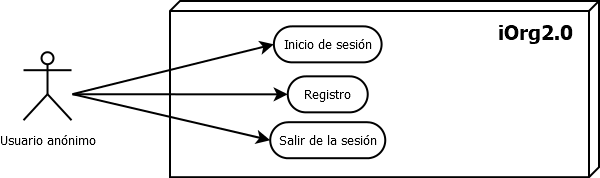
\includegraphics[width=1\textwidth]{../images/cu_anonimo.png}
  \caption{Diagrama de casos de uso actor usuario anónimo.}
  \label{fig:cu_anonimo}
  \end{center}
\end{figure}



\begin{figure}[!ht]
  \begin{center}
  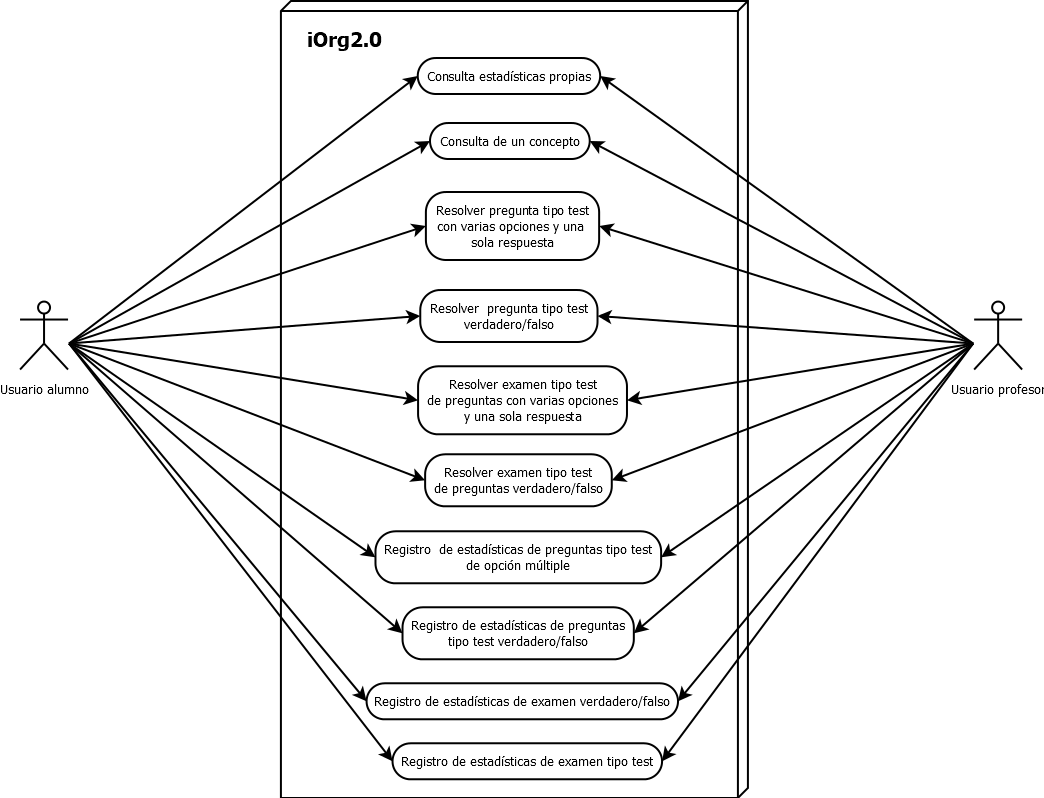
\includegraphics[width=1\textwidth]{../images/cu_alumno_profesor.png}
  \caption{Diagrama de casos de uso actores alumno y profesor.}
  \label{fig:cu_alumno_profesor}
  \end{center}
\end{figure}



\begin{figure}[!ht]
  \begin{center}
  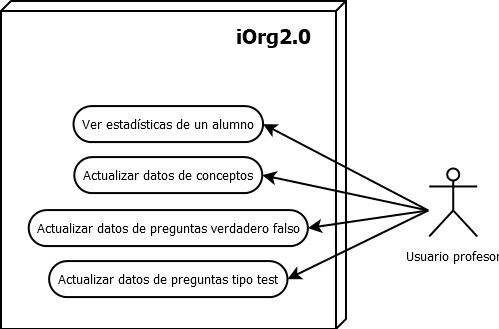
\includegraphics[width=1\textwidth]{../images/cu_profesor.png}
  \caption{Diagrama de casos de uso actor profesor.}
  \label{fig:cu_profesor}
  \end{center}
\end{figure}

\begin{figure}[!ht]
  \begin{center}
  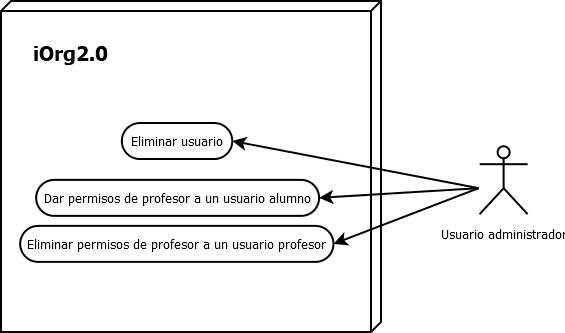
\includegraphics[width=1\textwidth]{../images/cu_administrador.png}
  \caption{Diagrama de casos de uso actor administrador.}
  \label{fig:cu_administrador}
  \end{center}
\end{figure}




\newpage

\section{Diagrama de navegación}
\bigskip
Aunque las secciones de esta aplicación no se preveen extensas en profundidad no está de más tener un diagrama donde mostrar la navegación:

\begin{figure}[!ht]
  \begin{center}
    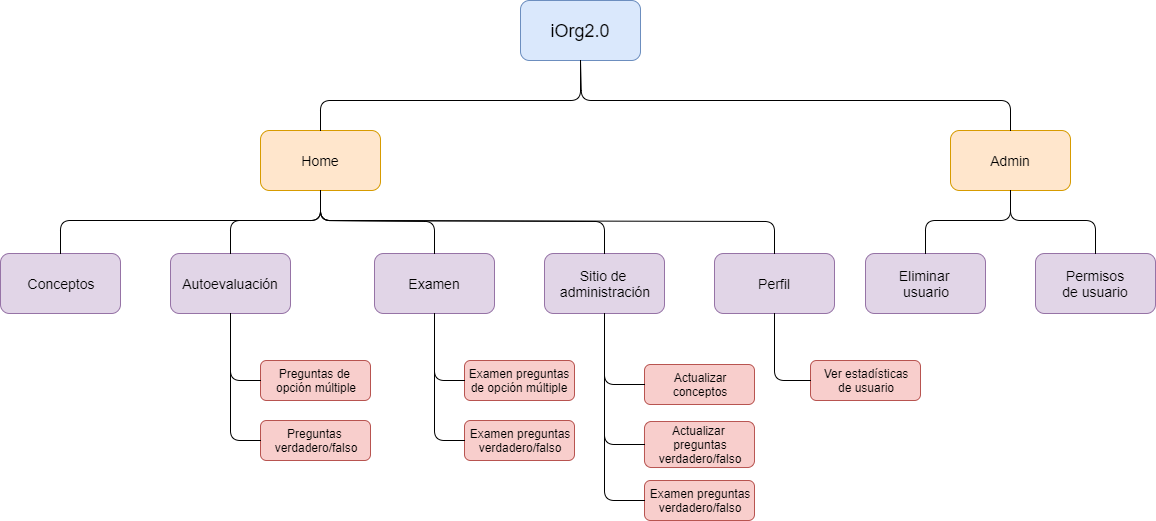
\includegraphics[width=1\textwidth]{../images/diagrama_navegacion.png}
    \caption{Diagrama de navegación}
    \label{fig:diagrama_navegacion}
  \end{center}
\end{figure}


